%
% slides-LaTeX-impatech-2025.tex
%
% Introdução ao LaTeX no IMPA Tech
%
% 2025 Rafael Luis Beraldo
% <rafael.beraldo@impatech.org.br>
%
%

\documentclass[numbering=fraction,aspectratio=169]{beamer}


% -------------------------------
% Pacotes
% -------------------------------
\usepackage{fontspec}
  \setmainfont{Latin Modern Roman}
  \newfontfamily\emoji{NotoColorEmoji}[Renderer=HarfBuzz]
\usepackage{polyglossia}
  \setdefaultlanguage[variant=brazilian]{portuguese}
\usepackage{hyperref}
\usepackage{xspace}
\usepackage{graphicx}
\usepackage{multicol}
\usepackage{microtype}
\usepackage{minted}
\usepackage{tcolorbox}
\usepackage{enumitem}

% -------------------------------
% Tema e estilo
% -------------------------------
\usetheme[progressbar=frametitle]{metropolis}
\beamertemplatenavigationsymbolsempty

% Cores
\definecolor{impatechpink}{RGB}{254,137,239}
\definecolor{impatechorange}{RGB}{254,196,84}
\definecolor{impatechgreen}{RGB}{189,255,139}

% Logo na caa
\titlegraphic{
\includegraphics[width=3cm]{img/impatech-logo}}

% Tema de cores e ajustes de fonte
\setbeamercolor{frametitle}{fg=black, bg=impatechorange}
\setbeamercolor{title separator}{fg=impatechorange}

\setbeamercolor{block title alerted}{fg=black, bg=impatechpink}
\setbeamercolor{block body alerted}{fg=black, bg=impatechpink!30}
\setbeamercolor{alerted text}{fg=impatechpink}
\setbeamerfont{alerted text}{series=\bfseries}

\setbeamercolor{block title example}{fg=black, bg=impatechgreen}
\setbeamercolor{block body example}{fg=black, bg=impatechgreen!30}
\setbeamercolor{footline}{fg=gray}
\setbeamercolor{progress bar}{fg=black}

% Rodapé
\setbeamertemplate{frame footer}{\insertshortauthor~(\insertshortinstitute)}


% -------------------------------
% Meus comandos
% -------------------------------
% IMPA Tech logo com pequeno espaçamento
\newcommand\IMPATech{\textsc{impa}\,Tech\xspace}
% Emoji
\newcommand\ThumbsUp{{\emoji 👍}\ }
\newcommand\ThumbsDown{{\emoji 👎}\ }
\newcommand\WarningEmoji{{\emoji ⚠️}\ }
% Itens semânticos
\newcommand{\filename}[1]{\texttt{#1}}
\newcommand{\email}[1]{\href{mailto:#1} {\texttt{\textless#1\textgreater}}}
% TODO
\newcommand{\todo}[1]{\colorbox{yellow}{#1}}
% Código
\newcommand{\code}[1]{\texttt{#1}}
\newmintinline[latexcode]{latex}{}

% -------------------------------
% URLs
% -------------------------------
% \def


% -------------------------------
% Metadados do título
% -------------------------------
\title{Introdução ao \LaTeX: dia três}
\author[Rafael Beraldo]{Rafael Luis Beraldo\\
  \texttt{<\href{mailto:rafael.beraldo@impatech.org.br}{rafael.beraldo@impatech.org.br}>}\\
  \textbf{Introdução ao \LaTeX}}
\institute{\IMPATech}
\date{24 de junho de 2025}


% -------------------------------
% Documento
% -------------------------------
\begin{document}
\frenchspacing

% Título
\begin{frame}[plain]{}
  \maketitle
\end{frame}

% Conteúdo
\begin{frame}
  \frametitle{Conteúdo}
  \setbeamertemplate{section in toc}[sections numbered]
  \begin{multicols}{2}
    \tableofcontents
  \end{multicols}
\end{frame}

% História %%%%%%%%%%%%%
\section{História}

\begin{frame}[plain]
  \begin{figure}[h]
    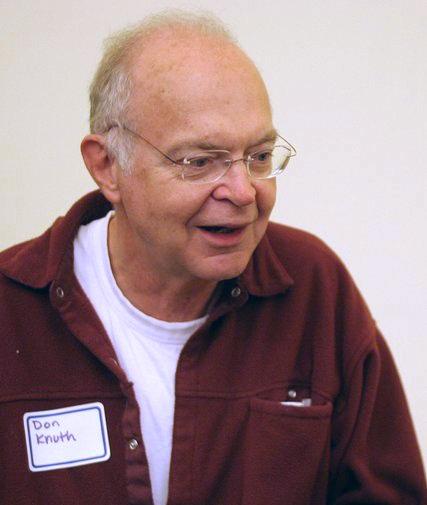
\includegraphics[scale=.5]{img/knuth}
    \caption{Donald Knuth em 2005}
  \end{figure}
\end{frame}

\begin{frame}[plain]
  \hspace*{-10.5mm}
  \centering
  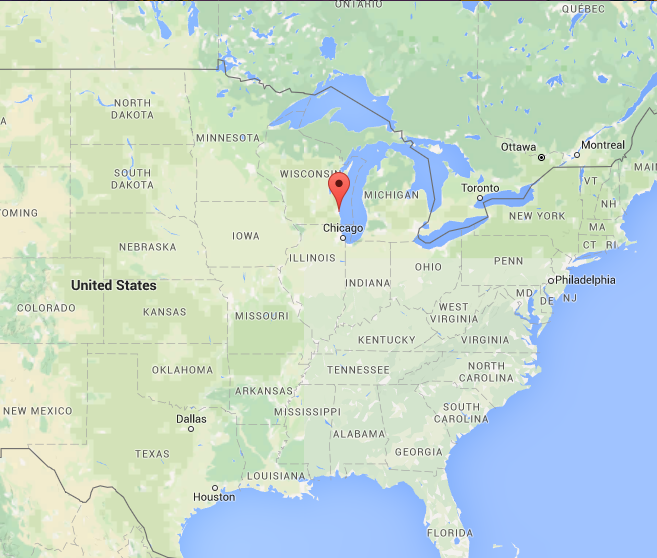
\includegraphics[width=\pagewidth]{img/milwaukee}
\end{frame}

\begin{frame}
  \frametitle{História do LaTeX}
  \LARGE
  \only<1>{O pai de Knuth tinha uma editora}
  \only<2>{1977: segunda edição do segundo volume de \emph{The Art of Computer Programming}}
  \only<3>{\textsc{ascii} não foi projetado com livros em mente}
  \only<4>{\TeX: tau epsilon chi}
\end{frame}

\begin{frame}
  \large
  \begin{quote}
    The purpose of this pronunciation exercise is to remind you that \TeX\ is primarily concerned with high-quality technical manuscripts: Its emphasis is on art and technology, as in the underlying Greek word. If you merely want to produce a passably good document—something acceptable and basically readable but not really beautiful—a simpler system will usually suffice. With \TeX\ the goal is to produce the finest quality; this requires more attention to detail, but you will not find it much harder to go the extra distance, and you’ll be able to take special pride in the finished product.\hfill (Donald Knuth, \emph{\TeX book})
  \end{quote}
\end{frame}

\begin{frame}
  \frametitle{História do LaTeX}
  \LARGE
  \LaTeX: 1985
\end{frame}

\begin{frame}[plain]
  \begin{figure}[h]
    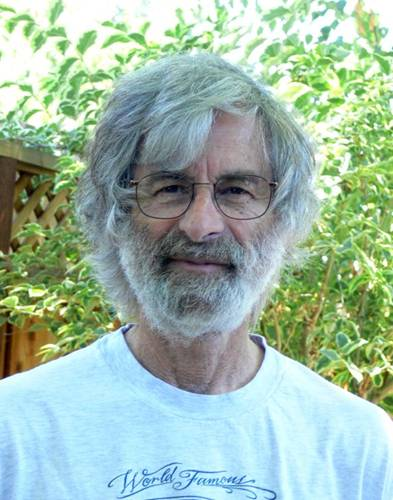
\includegraphics[scale=.5]{img/lamport}
    \caption{Leslie Lamport}
  \end{figure}
\end{frame}

% LaTeX: uma linguagem de marcação %%%%%%%%%%%%%%
\section[\LaTeX: uma linguagem de marcação]{Linguagem de marcação}

% O LaTeX é uma linguagem de marcação de texto, ou markup
\begin{frame}
  \frametitle{\LaTeX: uma linguagem de marcação}
  \LARGE
  \only<1>{\LaTeX{} é uma linguagem de \emph{markup}}
  \only<2>{Você \emph{declara} o documento}
  \only<3>{O programa segue as instruções}
  \only<4>{Assim como em \textsc{html}, o arquivo fonte é renderizado}
  \only<5>{Comandos são semânticos}
\end{frame}

% Se os comandos são semânticos, devem ser fáceis de interpretar. O que os
% comandos abaixo significam?
\begin{frame}[fragile]
  \frametitle{\LaTeX: uma linguagem de marcação}
  \begin{minted}[autogobble,fontsize=\LARGE,breaklines]{latex}
    \tableofcontents

    \section{Introdução}
  \end{minted}
\end{frame}

% Arquivos .tex não contém formatação; são texto plano.
\begin{frame}
  \frametitle{\LaTeX: uma linguagem de marcação}
  \LARGE
  \code{.tex} são arquivos de texto plano
\end{frame}

% Exemplo de artigo %%%%%%%%%%%%%%
\section{Exemplo de artigo}

% Vejamos nosso primeiro artigo em LaTeX.
\begin{frame}
  \frametitle{Exemplo de artigo}
  \Huge
  Vejamos \filename{exemplos/artigo.tex}
\end{frame}

% Comandos %%%%%%%%%%%%%%
\section{Comandos}

% Comandos simples não têm argumentos
\begin{frame}[fragile]
  \frametitle{Comandos simples}
  \begin{minted}[autogobble,fontsize=\LARGE,breaklines]{latex}
    \tableofcontents
  \end{minted}
\end{frame}

% Comandos simples e espaço em branco
\begin{frame}[fragile]
  \frametitle{Comandos simples e espaço em branco}
  \begin{minted}[autogobble,fontsize=\LARGE,breaklines]{latex}
    \tableofcontents Isso funciona
  \end{minted}
\end{frame}

\begin{frame}[fragile]
  \frametitle{Comandos simples e espaço em branco}
  \begin{minted}[autogobble,fontsize=\LARGE,breaklines]{latex}
    \tableofcontents
    Melhor agora
  \end{minted}
\end{frame}

% Comandos com argumentos
\begin{frame}[fragile]
  \frametitle{Comandos com argumento}
  \begin{minted}[autogobble,fontsize=\normalsize,breaklines]{latex}
    \section{Introdução}\label{introducao}Também funciona
  \end{minted}
\end{frame}

% Voltemos ao exemplo para demonstrar
\begin{frame}
  \frametitle{Exemplos de comandos}
  \huge
  Vejamos \filename{exemplo/artigo.tex} novamente
\end{frame}

%
% espaco-branco.tex
%
% Introdução ao LaTeX no IMPA Tech
%
% 2025 Rafael Luis Beraldo
% <rafael.beraldo@impatech.org.br>
%
% Problema: o espaçamento deste texto está catastrófico. Existem espaços
% sobrando ou faltando, tanto entre as palavras quanto entre os parágrafos. O
% texto final deve conter quatro parágrafos, sendo o segundo uma lista cujos
% itens são separados por novas linhas. Corrija os problemas e compile o
% documento.
%

\documentclass{article}
\begin{document}
Acima de tudo, é fundamental ressaltar que o julgamento imparcial das eventualidades maximiza as possibilidades por conta das direções preferenciais no sentido do progresso. Desta maneira,a complexidade dos estudos efetuados cumpre um papel essencial na formulação das condições financeiras e administrativas                       exigidas, que são três:
1. O mundo atual.
2. Os amigos de família.
3. A importância dos mercados mundiais.
Nunca é demais lembrar o peso e o significado destes problemas, uma vez que o fenômeno da Internet exige a precisão e a definição do processo de comunicação como um todo. No entanto, não podemos esquecer que                    a consulta aos diversos militantes agrega valor ao estabelecimento das regras de conduta normativas.Do mesmo modo, o acompanhamento das preferências de consumo garante a contribuição de um grupo importante na determinação das novas proposições.
O empenho em analisar o desenvolvimento contínuo de distintas formas de atuação aponta para a melhoria do sistema de participação geral.  Neste sentido, a competitividade nas transações comerciais desafia a capacidade de equalização dos relacionamentos verticais entre as hierarquias. É importante questionar o quanto o início da atividade geral de formação de atitudes facilita a criação das diretrizes de desenvolvimento para o futuro. Evidentemente, a execução dos pontos do programa promove a alavancagem do retorno esperado a longo prazo.
\end{document}

% Símbolos especiais %%%%%%%%%%%%%%
\section{Símbolos especiais}

% Aspas
\begin{frame}[fragile]
  \frametitle{Aspas}
  \begin{minted}[autogobble,fontsize=\LARGE,breaklines]{latex}
    ``Devemos abrir aspas com dois acentos graves e fechar com duas aspas
    simples.''
  \end{minted}
\end{frame}

% Traços
\begin{frame}[fragile]
  \frametitle{Hífen, travessão e meia-risca}
  \begin{minted}[autogobble,fontsize=\LARGE,breaklines]{latex}
    Leve um guarda-chuva --- ouvi na rádio que pode chover entre 10h--13h.
  \end{minted}
\end{frame}

% Espaços não quebráveis
\begin{frame}[fragile]
  \frametitle{Espaços não quebráveis}
  \begin{minted}[autogobble,fontsize=\LARGE,breaklines]{latex}
    Às 10~horas de ontem…
    Fui à casa do Sr.~Silva…
    Veja mais na página~40.
  \end{minted}
\end{frame}

% Os símbolos a seguir são especiais e devem ser escapados:
\begin{frame}[fragile]
  \frametitle{Caracteres reservados}
  \begin{minted}[autogobble,fontsize=\LARGE,breaklines]{latex}
    # $ % ^ & _ { } ~ \

    \# \$ \% \^{} \& \_ \{ \} \~{} \textbackslash
  \end{minted}
\end{frame}

% Resolver o exercício
\begin{frame}
  \frametitle{Caracteres reservados}
  \huge
  Resolver \filename{exercicios/caracteres-reservados.tex}
\end{frame}

% Preambulo do documento %%%%%%%%%%%%%%
\section{Preâmbulo do documento}

% Dar uma olhada no arquivo. Ensinar a distinção entre o preâmbulo e o corpo do
% documento.
\begin{frame}
  \frametitle{Preâmbulo do documento}
  \LARGE
  Documentos \LaTeX: preâmbulo e corpo
\end{frame}

\begin{frame}[fragile]
  \frametitle{Preâmbulo do documento}
  \LARGE
  \begin{minted}[autogobble,fontsize=\large,breaklines]{latex}
  \documentclass[11pt,a4paper,oneside]{article}
  \end{minted}
\end{frame}

% Explicar as opções da classe article que escolhi
\begin{frame}[fragile]
  \frametitle{Preâmbulo do documento}
  \LARGE
  Classes padrão:
  \begin{multicols}{2}
    \begin{itemize}
      \item\code{article}
      \item\code{report}
      \item\code{book}
      \item\code{letter}
      \item\code{memoir}
      \item\code{beamer}
  \end{itemize}
\end{multicols}
\end{frame}

% Vejamos quais são as opções de classe mais comuns
\begin{frame}
  \frametitle{Preâmbulo do documento}
  \LARGE
  Opções de classe comuns:
  \begin{itemize}
    \only<1>{\item \code{10pt, 11pt, 12pt}}
    \only<1>{\item \code{a4paper, a5paper, letterpaper, …}}
    \only<2>{\item \code{titlepage, notitlepage}}
    \only<2>{\item \code{twocolumn}}
    \only<2>{\item \code{twoside, oneside}}
    \only<3>{\item \code{landscape}}
    \only<3>{\item \code{openright, openany}}
    \only<3>{\item \code{draft}}
  \end{itemize}
\end{frame}

\begin{frame}
  \frametitle{Preâmbulo do documento}
  \huge
  Vejamos \filename{exemplos/artigo.tex}
\end{frame}

% Corpo do documento %%%%%%%%%%%%%%
\section{Corpo do documento}

% O corpo do documento
\begin{frame}[fragile]
  \frametitle{Corpo do documento}
  \begin{minted}[autogobble,fontsize=\LARGE,breaklines]{latex}
    \begin{document}
     …
    \end{document}
  \end{minted}
\end{frame}

% Divisões do documento
\begin{frame}[fragile]
  \frametitle{Corpo do documento: divisões do documento}
  \large
  \begin{multicols}{2}
    \begin{itemize}
      \item\latexcode{\part} (-1)
      \item\latexcode{\chapter} (0)
      \item\latexcode{\section} (1)
      \item\latexcode{\subsection} (2)
      \item\latexcode{\subsubsection} (3)
      \item\latexcode{\paragraph} (4)
      \item\latexcode{\subparagraph} (5)
    \end{itemize}
  \end{multicols}
\end{frame}

% Profundidade
\begin{frame}[fragile]
  \frametitle{Corpo do documento: profundidade das divisões}
  \begin{minted}[autogobble,fontsize=\LARGE,breaklines]{latex}
  \setcounter{secnumdepth}{3}
  \setcounter{tocdepth}{3}
  \end{minted}
\end{frame}

% Comandos estrelados para controlar numeração e o que vai no sumário
\begin{frame}[fragile]
  \frametitle{Corpo do documento: comandos estrelados}
  \begin{minted}[autogobble,fontsize=\large,breaklines]{latex}
  \section*{Esta seção não terá numeração nem aparecerá no sumário}
  \end{minted}
\end{frame}

% Sintaxe para controlar título que vai no sumário
\begin{frame}[fragile]
  \frametitle{Corpo do documento: controlar texto do sumário}
  \begin{minted}[autogobble,fontsize=\large,breaklines]{latex}
  \section[Seção muito longa]{Seção muito longa: provavelmente não ficará muito boa no sumário.}
  \end{minted}
\end{frame}

\begin{frame}
  \frametitle{Corpo do documento: parágrafos}
  \LARGE
  Parágrafos são separados\\
  por linhas em branco
\end{frame}

\begin{frame}[fragile]
  \frametitle{Corpo do documento: espaçamento entre parágrafos}
  \begin{minted}[autogobble,fontsize=\LARGE,breaklines]{latex}
  \setlength{\parskip}{1cm}
  \setlength{\parskip}{1cm plus4mm minus3mm}
  \end{minted}
\end{frame}

\begin{frame}
  \frametitle{Corpo do documento: indentação}
  \LARGE
  Pacote \code{indentfirst}
\end{frame}

\begin{frame}
  \frametitle{Corpo do documento}
  \huge
  Vejamos \filename{exemplo/artigo.tex}
\end{frame}

\begin{frame}
  \frametitle{Corpo do documento}
  \huge
  Resolver \filename{exercicios/meu-artigo.tex}
\end{frame}

%
% pacotes.tex
%
% Introdução ao LaTeX no IMPA Tech
%
% 2025 Rafael Luis Beraldo
% <rafael.beraldo@impatech.org.br>
%
% Problema: adicione o pacote polyglossia após a linha 10, configure o idioma
% português e compile.
%

\documentclass{article}
\begin{document}
  Muito além, nos confins inexplorados da região mais brega da
  Borda Ocidental desta Galáxia, há um pequeno sol amarelo e esquecido.

  Girando em torno deste sol, a uma distância de cerca de 148~milhões de
  quilômetros, há um planetinha verde-azulado absolutamente insignificante.
\end{document}

% Fontes %%%%%%%%%%%%%%
\section{Fontes}

% O pdflatex é mais limitado e, por isso, utilizaremos o lualatex
\begin{frame}
  \frametitle{Fontes}
  \LARGE
  \code{pdflatex} não suporta todas as fontes, portanto usamos \code{lualatex}
\end{frame}

% O pacote fontspec é carregado automaticamente pelo polyglossia, mas
% carregaremos ele mesmo assim.
\begin{frame}[fragile]
  \frametitle{Fontes}
  \LARGE
  Aproveitar as vantagens do Unicode:
  \begin{minted}[autogobble,fontsize=\LARGE,breaklines]{latex}
    \usepackage{fontspec}
      \setmainfont{Times New Roman}
  \end{minted}
\end{frame}

% Exemplo do que podemos fazer usando LaTeX e Unicode. É claro, a fonte tem que
% conter os caracteres que estamos tentando usar.
\begin{frame}
  \frametitle{Fontes}
  \LARGE
  Εὐριπίδης — meu amigo de tantos anos — só lê Достое́вский.
\end{frame}

% Vamos aprender a acessar os diversos tipos de uma família de fontes. Vamos
% discutir com mais profundidade no exemplo e exercício.
\begin{frame}[fragile]
  \frametitle{Fontes e seus tipos}
  \LARGE
  \only<1>{Fontes vêm em famílias}
  \only<2>{\latexcode{\textrm}: \textrm{romanas}}
  \only<3>{\latexcode{\emph}: \emph{ênfase}}
  \only<4>{\latexcode{\textbf}: \textbf{negrito}}
  \only<5>{\latexcode{\textsc}: \textsc{Versaletes}}
  \only<6>{\latexcode{\texttt}: \texttt{teletipo}}
\end{frame}

% Tamanhos de fontes em LaTeX. Geralmente não é uma boa ideia usar eles à mão,
% pois os designers das classes de documento tomam essas decisões para nós.
\begin{frame}[fragile]
  \frametitle{Fontes}
  \large
  Tamanhos de fonte:
  \begin{multicols}{2}
    \begin{itemize}
      \item{\code{\textbackslash tiny}: 5pt}
      \item{\code{\textbackslash scriptsize}: 7pt}
      \item{\code{\textbackslash footnotesize}: 8pt}
      \item{\code{\textbackslash small}: 9pt}
      \item{\code{\textbackslash normalsize}: 10pt}
      \item{\code{\textbackslash large}: 12pt}
      \item{\code{\textbackslash Large}: 14pt}
      \item{\code{\textbackslash LARGE}: 17pt}
      \item{\code{\textbackslash huge}: 20pt}
      \item{\code{\textbackslash Huge}: 25pt}
    \end{itemize}
  \end{multicols}
\end{frame}

\begin{frame}
  \frametitle{Fontes}
  \begin{quote}
    \underline{\textbf{Remember\Huge!}} \textit{The}
    \textsf{M\textbf{\LARGE O} \texttt{R}\textsl{E}} fonts \Huge you
    \tiny use \footnotesize \textbf{in} a \small \texttt{document},
    \large \textit{the} \normalsize more \textsc{readable} and
    \textsl{\textsf{beautiful} it bec\large o\Large m\LARGE e\huge s}.
  \end{quote}
  \begin{flushright}
    (\texttt{lshort.pdf}, p. 188)
  \end{flushright}
\end{frame}

% Como trocar as fontes. Explicar que fontes matemáticas são outra história.
\begin{frame}[fragile]
  \frametitle{Fontes}
  \large
  Carregar fontes usando o \code{fontspec}:

  \begin{minted}[autogobble,fontsize=\Large,breaklines]{latex}
    \usepackage{fontspec}
      \setmainfont{Linux Libertine}
  \end{minted}
\end{frame}

% Fontes devem estar nos diretórios padrão. Caso não estejam, podemos
  % especificar um diret´orio:
\begin{frame}[fragile]
  \frametitle{Fontes}
  \Large
  Especificar um diretório:

  \begin{minted}[autogobble,fontsize=\Large,breaklines]{latex}
    \usepackage{fontspec}
      \setmainfont{Linux Libertine}[
        Path = fonts/
      ]
  \end{minted}
\end{frame}

% Ligaduras são sequências de letras que naturalmente colidem. Por isso, são
% substituídas por outro caractere.
\begin{frame}
  \frametitle{Fontes}
  \LARGE
  Linux Libertine e ligaduras

  \fontspec{Linux Libertine}{
    affair\qquad fjord\qquad flor\\
    af\mbox{}fair\qquad f\mbox{}jord\qquad f\mbox{}lor
  }
\end{frame}

% Antes do exercício, vamos rever os conceitos que discutimos de maneira
% prática.
\begin{frame}
  \frametitle{Fontes}
  \huge
  Demonstrar ideias em \filename{exemplos/fontes.tex}
\end{frame}

% Resolver o exercício fontes-exercicio.tex.
\begin{frame}
  \frametitle{Fontes}
  \huge
  Resolver \filename{exercicios/sonhos-noite-verao.tex}
\end{frame}

%
% layouts-pagina.tex
%
% Introdução ao LaTeX no IMPA Tech
%
% 2025 Rafael Luis Beraldo
% <rafael.beraldo@impatech.org.br>
%
% Demonstra:
% - Margens com as opções onecolumn and twocolumn
% - Visualização de margens com o pacote showframe
% - O pacote fullpage e seus problemas
% - O pacote setspace e a entrelinha
% - Estilos de página
%
% O documento está vazio, pois depende da solução de sonhos-noite-verao.tex.

%
% posicao-texto.tex
%
% Introdução ao LaTeX no IMPA Tech
%
% 2025 Rafael Luis Beraldo
% <rafael.beraldo@impatech.org.br>
%
% Demonstra:
% - Ambientes center, flushleft e flushright
% - Como controlar o espaço horizontal e vertical com \hspace, \vspace, \hfill
%   e \vfill
% - Diferentes unidades que o LaTeX conhece
%

\documentclass[a4paper]{article}
\usepackage{fontspec}
\usepackage{polyglossia}
  \setdefaultlanguage{brazil}

\begin{document}
\frenchspacing

\section{Ambientes}

Para posicionar o texto horizontalmente na página, podemos usar três
\textbf{ambientes}: \texttt{center, flushleft} e \texttt{flushright}.

\begin{center}
  Todo este texto será centralizado na página.
\end{center}

\begin{flushleft}
  Esse parágrafo será alinhado à esquerda e não será justificado. Mais abaixo,
  veremos como ajustar a posição de um texto dentro da própria linha.
\end{flushleft}

\begin{flushright}
  Também podemos alinhar texto à direita. Além desses ambientes, podemos mudar
  o alinhamento do texto usando os comandos \verb+\centering+,
  \verb+\flushleft+ e \verb+\flushright+.
\end{flushright}

\section{Controlando o espaço na linha}

Os comandos \verb+\hspace{comprimento}+ e \verb+\hfill+ nos permitem controlar
o espaço dentro de uma linha:

Aqui haverá\hspace{1.5cm} um espaço.

Começo\hfill meio\hfill fim.

\section{Espaço vertical}

Os comandos para controle do espaço vertical, isto é, o espaço entre os
parágrafos, são muito parecidos com os comandos de espaço horizontal. Eles são
\verb+\vspace{comprimento}+ e \verb+\vfill+.
\end{document}

% Listas %%%%%%%%%%%%%%
\section{Listas}

% Três tipos de listas inclusos por padrão
\begin{frame}
  \frametitle{Listas: três tipos}
  \LARGE
  Ambientes: \code{itemize, enumerate} e \code{description}
\end{frame}

% Anatomia de uma lista
\begin{frame}[fragile]
  \frametitle{Listas: sintaxe}
  \Large
  Ingredientes para carbonara:

  \begin{minted}[autogobble,fontsize=\Large,breaklines]{latex}
    \begin{itemize}
      \item Bacon
      \item Macarrão
      \item Ovos
      \item Parmesão
      \item Pimenta-do-reino
    \end{itemize}
  \end{minted}
\end{frame}

% Existem mais listas no arquivo exemplos/listas.tex
\begin{frame}
  \frametitle{Listas: exemplo}
  \Huge
  Aprenderemos mais em \filename{exemplos/listas.tex}
\end{frame}

% Exercício: completar a receita de panqueca com os ingredientes corretos.
\begin{frame}
  \frametitle{Listas: exercício}
  \Huge
  Resolver \filename{exercicios/receita.tex}
\end{frame}

% Lista de ingredientes que os participantes devem colocar na receita. Notar a
% palavra ingrediente, o número sequencial e o parênteses.
\begin{frame}
  \frametitle{Listas: exercício}

  \begin{enumerate}[label=Ingrediente \arabic*), leftmargin=3cm]
    \item 190g de farinha
    \item 25g de açúcar
    \item 10g de fermento químico em pó
    \item 3g de sal\\[0.8ex] … texto …\\[0.8ex]
    \item 25g de manteiga\\[0.8ex] … texto …\\[0.8ex]
    \item 330g de leite
    \item 80g de ovos
  \end{enumerate}
\end{frame}

% Tabelas %%%%%%%%%%%%%%
\section{Tabelas}

\begin{frame}
  \frametitle{Tabelas}
  \LARGE
  A abordagem é diferente\\
  dos programas WISIWYG
\end{frame}

% Exemplo simples de tabela com o ambiente tabular
\begin{frame}[fragile]
  \frametitle{Tabelas: exemplo simples}
  \LARGE
  Exemplo do ambiente \code{tabular}:
  \vspace{1em}

  \begin{minipage}{.65\textwidth}
    \begin{minted}[autogobble,fontsize=\Large,breaklines]{latex}
      \begin{tabular}{lcr}
        1 & 2 & 3\\
        4 & 5 & 6\\
        7 & 8 & 9
      \end{tabular}
    \end{minted}
  \end{minipage}
  \hspace{.05\textwidth}
  \begin{minipage}{.25\textwidth}
    \begin{tabular}{lcr}
      1 & 2 & 3\\
      4 & 5 & 6\\
      7 & 8 & 9
    \end{tabular}
  \end{minipage}
\end{frame}

% Com mais alguns detalhes como linhas verticais e horizontais
\begin{frame}[fragile]
  \frametitle{Tabelas: linhas}
  \LARGE
  Linhas horizontais e verticais:
  \vspace{1em}

  \begin{minipage}{.65\textwidth}
    \begin{minted}[autogobble,fontsize=\Large,breaklines]{latex}
      \begin{tabular}{l|c|r}
        \hline
        1 & 2 & 3\\
        4 & 5 & 6\\
        7 & 8 & 9\\
        \hline
      \end{tabular}
    \end{minted}
  \end{minipage}
  \hspace{.05\textwidth}
  \begin{minipage}{.25\textwidth}
    \begin{tabular}{l|c|r}
      \hline
      1 & 2 & 3\\
      4 & 5 & 6\\
      7 & 8 & 9\\
      \hline
    \end{tabular}
  \end{minipage}
\end{frame}

% O espaço em branco deixa o texto respirar e evita a tirania das linhas retas.
% Essa citação do Bringhurst é fantástica.
\begin{frame}
  \frametitle{Tabelas: espaço branco}
  \large
  \begin{quote}
    Assim como o texto, as tabelas ficam canhestras quando abordadas de forma
    puramente técnica. Boas soluções tipográficas não costumam surgir em resposta
    a perguntas do tipo “Como posso enfiar essa quantidade de caracteres naquele
    tanto de espaço?”.\\[1em]

    (Robert Bringhurst, \emph{Elementos do Estilo Tipográfico)}
  \end{quote}
\end{frame}

% Vejamos alguns exemplos
\begin{frame}
  \frametitle{Tabelas: exemplo}
  \Huge
  Vejamos \filename{exemplos/tabelas.tex}
\end{frame}

% Vamos revisar o que aprendemos no exemplo.
\begin{frame}[fragile]
  \frametitle{Tabelas: revisão}
  \LARGE
  Aprendemos:

  \begin{itemize}
    \only<1>{\item \code{tabular}}
    \only<1>{\item tipografia da tabela}
    \only<1>{\item quebras de linhas}
    \only<2>{\item \code{booktabs}}
    \only<2>{\item \latexcode{\multicolumn}}
    \only<2>{\item \code{longtable}}
  \end{itemize}
\end{frame}

% Temos declarado exatamente onde desejamos que a tabela fique, mas essa
% abordagem nem sempre é boa, porque interrompe o fluxo do texto. Vamos
% aprender mais sobre os ambientes do tipo float.
\begin{frame}
  \frametitle{Tabelas: floats}
  \LARGE
  \only<1>{Ambiente \code{tabular} coloca\\ a tabela após o texto}
  \only<2>{Padrão profissional: \emph{floats}}
  \only<3>{Dois floats: \code{table} e \code{figure}}
\end{frame}

% A sintaxe do ambiente table
\begin{frame}[fragile]
  \frametitle{Tabelas: \code{table}}
  \LARGE
  Sintaxe de \code{table}
  \vspace{1em}

    \begin{minted}[autogobble,fontsize=\LARGE,breaklines]{latex}
      \begin{table}[posição]
        …
      \end{table}
    \end{minted}

    \emph{(\code{tbp} é a posição padrão)}
\end{frame}

% Exemplo, com os comandos \centering, \caption e \label.
\begin{frame}[fragile]
  \frametitle{Tabelas: \code{table}}
  \large
  Veja a tabela~\ref{tab:numerosUmNove}:
  \vspace{1em}

  \begin{minipage}{.65\textwidth}
    \begin{minted}[autogobble,fontsize=\large,breaklines]{latex}
    \begin{table}
      \centering
      \begin{tabular}{lcr}
      1 & 2 & 3\\
      4 & 5 & 6\\
      7 & 8 & 9
      \end{tabular}
      \caption{Números de 1 a 9}
      \label{tab:numerosUmNove}
    \end{table}
    \end{minted}
  \end{minipage}
  \hspace{.05\textwidth}
  \begin{minipage}{.25\textwidth}
    \begin{table}
      \centering
      \begin{tabular}{lcr}
        1 & 2 & 3\\
        4 & 5 & 6\\
        7 & 8 & 9
      \end{tabular}
      \caption{Números de 1 a 9}
      \label{tab:numerosUmNove}
    \end{table}
  \end{minipage}
\end{frame}

% Voltaremos ao arquivo anterior para brincar com esses conceitos e
% referências cruzadas.
\begin{frame}
  \frametitle{Tabelas: exemplos de \code{table}}
  \Huge
  Voltemos à \filename{exemplos/tabelas.tex}
\end{frame}

% Exercício: uma tabela do zero, usando o ambiente table e referenciando a
% tabela num parágrafo anterior.
\begin{frame}
  \frametitle{Tabelas: exercício}
  \Huge
  Resolver: \filename{exercicios/robos.tex}
\end{frame}

% \begin{frame}
%   \frametitle{Tabelas: ferramentas}
%   \Huge
%   Mais recursos em \filename{conteudo.md}
% \end{frame}

%
% imagens.tex
%
% Introdução ao LaTeX no IMPA Tech
%
% 2025 Rafael Luis Beraldo
% <rafael.beraldo@impatech.org.br>
%
% Demonstra:
% - Como incluir gráficos com o pacote graphicx
% - Controlar o tamanho e escala dos gráficos
% - O ambiente figure
% - O ambiente minipage e seus usos
% - Outras capacidades do graphicx (ver documentação)
%

\documentclass[a4paper,oneside]{article}
\usepackage{fontspec}
\usepackage{polyglossia}
  \setdefaultlanguage{brazil}
\usepackage{graphicx}

\begin{document}
\frenchspacing

% Informação e imagem encontrados na Wikipédia em:
% https://en.wikipedia.org/wiki/Alpha_Centauri
\section{Nosso vizinhos}

Na figura~\ref{fig:estrelas}, podemos ver nossos vizinhos mais próximos, por
assim dizer. A estrela circulada é Proxima Centauri, uma pequena anã vermelha,
que pode estar ligada gravitacionalmente às outras duas estrelas. A olho nu, as
duas estrelas parecem uma só.

% Brincar os as opções de posicionamento do figure e de tamanho do
% \includegraphics. Ensinar o ambiente minipage, e a técnica de colocar dois
% minipages dentro de um figure para colocar uma imagem ao lado da outra.
\begin{figure}[h]
  \centering
  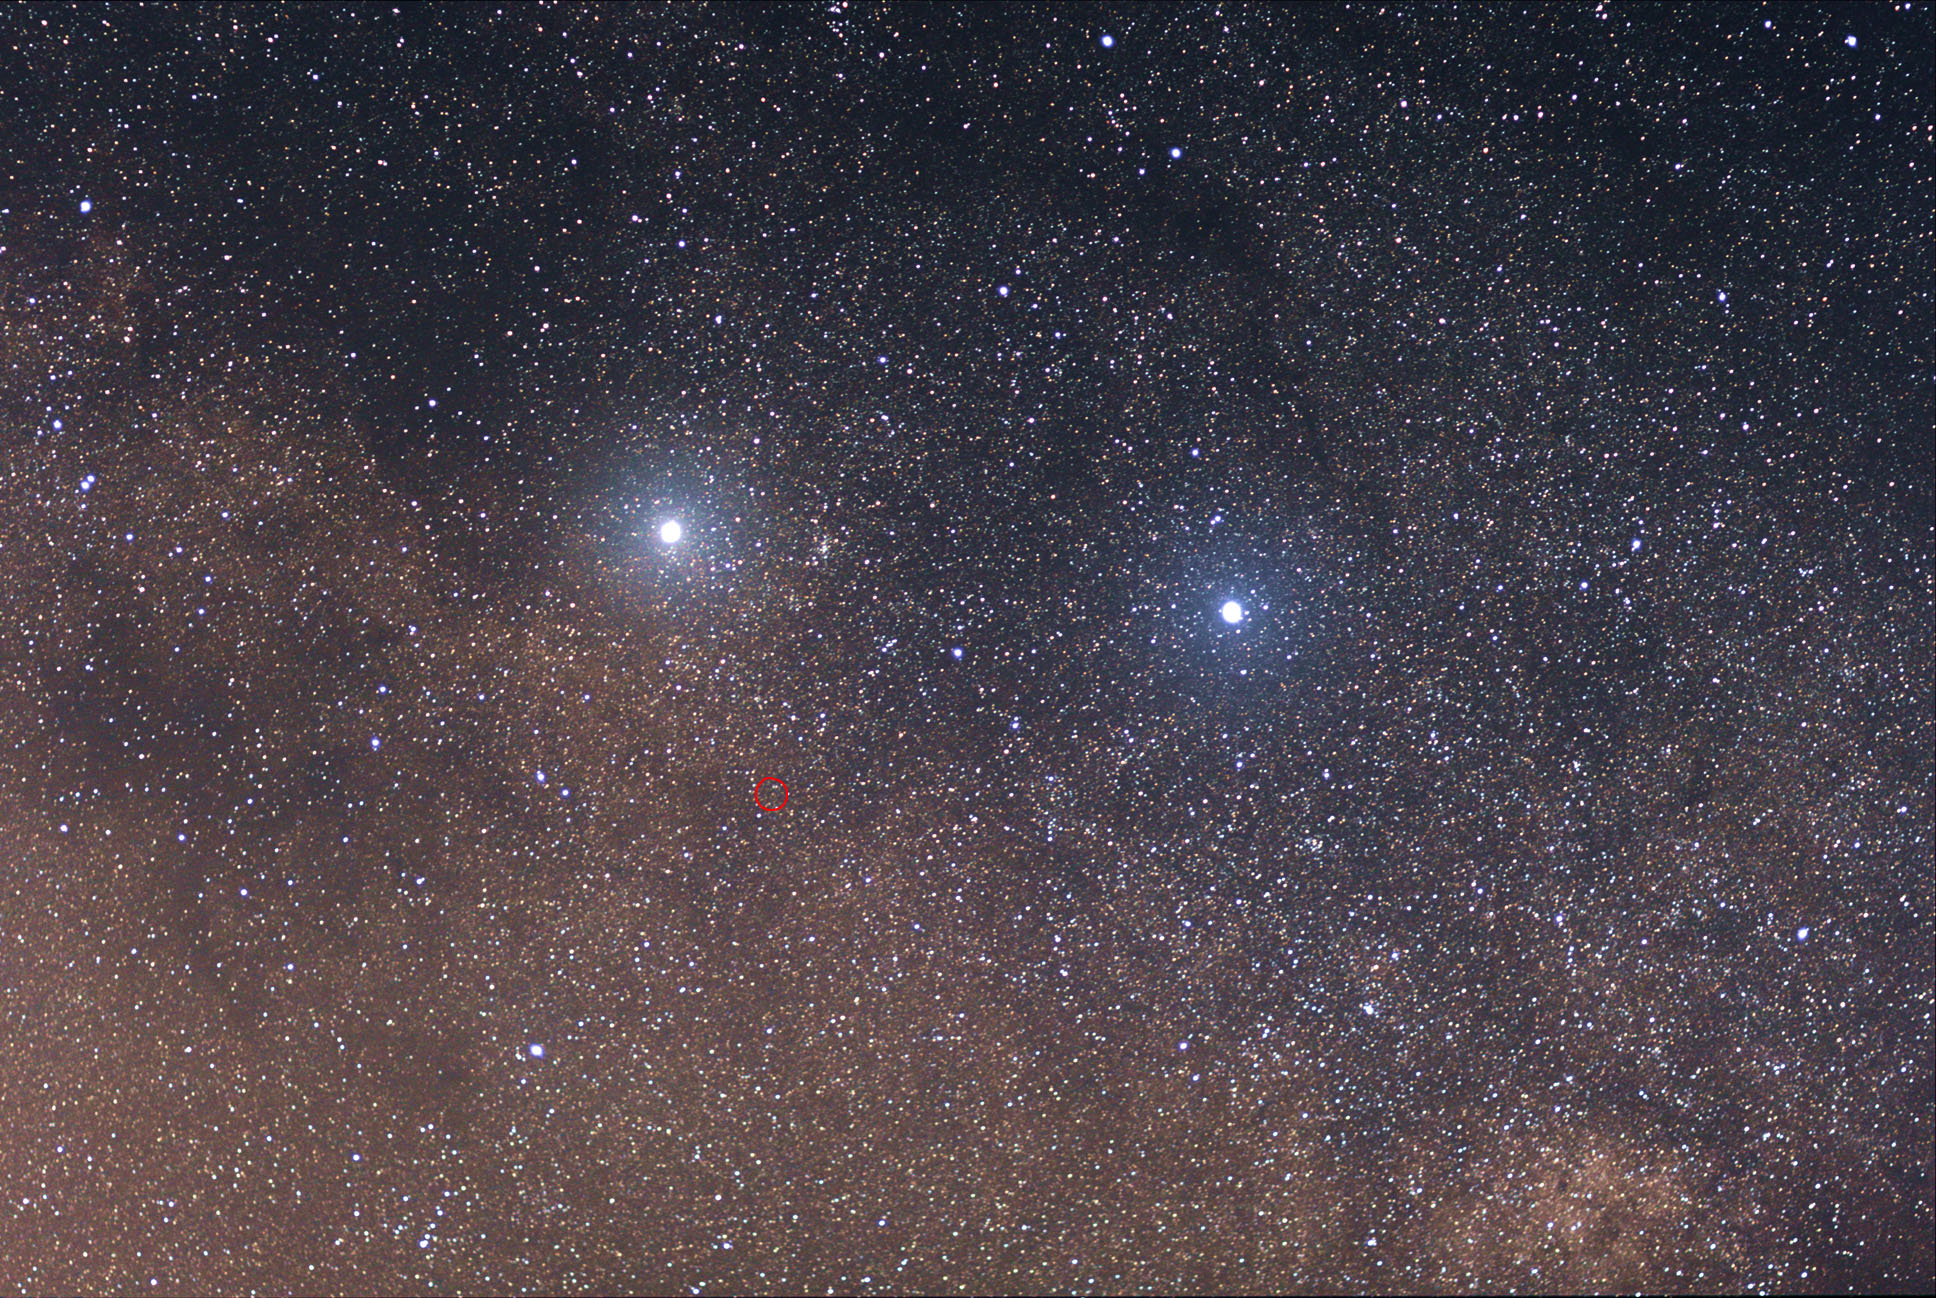
\includegraphics[width=\textwidth]{imagens/alpha-beta-proxima-centauri}
  \caption{Alpha Centauri e Beta Centauri, com Proxima circulada}
  \label{fig:estrelas}
\end{figure}
\end{document}

%
% matematica.tex
%
% Introdução ao LaTeX no IMPA Tech
%
% 2025 Rafael Luis Beraldo
% <rafael.beraldo@impatech.org.br>
%
% Demonstra:
% - Ambientes para inserir equações: math, displaymath e equation
% - Como inserir símbolos, letras gregas, operadores, potências e subscritos,
%   frações e raízes
%

\documentclass[a4paper,oneside]{article}
\usepackage{fontspec}
\usepackage{polyglossia}
  \setdefaultlanguage{brazil}
\usepackage{mathtools}

\begin{document}
\frenchspacing

\section{Três ambientes para matemática}

No \LaTeX, há três ambientes para acessar o modo de matemática. Eles são o
\texttt{math}, \texttt{displaymath} e \texttt{equation}. O primeiro é do tipo
\emph{inline} (o ambiente não cria um novo parágrafo), enquanto que os dois
últimos são do tipo \emph{displayed} (o ambiente cria um novo parágrafo).
É possível acessar o ambiente \texttt{math} usando o atalho \verb+\( … \)+ e o
ambiente \texttt{displaymath} é equivalente a \verb+\[ … \]+.

% Mostrar o efeito dos três ambientes discutidos acima, além dos comandos
% \label e \tag.
\bigskip
Newton demostrou que a força gravitacional entre dois objetos é igual a \( F =
G \frac{m_1 m_2}{r^2} \) em 1687, quando publicou o \emph{Principia}.

\section{Símbolos}

Há centenas de símbolos já implementados no LaTeX, além daqueles que você tem
acesso no seu teclado. Aqui estamos combinando os dois tipos:

\[ 2 \times 2 = 4 \]

No modo de matemática, o espaçamento funciona de maneira diferente. O LaTeX
automaticamente escolhe o espaçamento entre os símbolos, números etc. Por
exemplo:

\[ ab = ba \]

\section{Letras gregas}

É fácil acessar letras gregas:

\[ \text{Circunferência} = 2 \pi r \]

\section{Operadores}

De maneira similar, muitos operadores já estão implementados: \( \log xy = \log
x + \log y \).

Uma das formas de criptografia mais antigas é conhecida como a Cifra de César:

\begin{equation}
  E_n(x) = (x + n) \bmod 26
  \tag{Cifra de César}
\end{equation}

\section{Potências e subscritos}

Potências são representadas com acentos circunflexos, \( 2^8 \). Subscritos são
representados com underlines, \( a_b \). Como em muitos outros casos no modo de
matemática, é possível agrupar valores usando chaves: \( 2^{32} \).

\[ f(n) = 4n + n^2 \]

\section{Frações}

Frações podem ser usadas com o comando \verb+\frac+: \( \frac{2}{5} \). Também
é possível incluir frações dentro de frações:

\[ \frac{\frac{1}{x}+\frac{1}{y}}{y-z} \]

\section{Raízes}

Assim como no caso das frações, raízes têm um comando especial: \verb+\sqrt+.
A proporção \( 1:\sqrt{2} \) é usada frequentemente em tipografia. Também é
possível escrever raízes com expoentes diferentes:

\[ \sqrt[3]{27} = 3 \]
\end{document}


\end{document}

% Local Variables:
% jinx-languages: "pt_BR"
% End:
